% DONE! -tnetter 10/09/2009 16:02 
% ===============================
% Data collection
% ===============================
\newpage
\section{Data}
\label{sec:datacollection}

When gathering data for behavioral analysis of different species, the observer usually tracks the position of one or several individuals over time. Additionally, pheno- and genotypical data is collected about each individual.

Spatial position is usually recorded by one or several persons. In this project however, data is collected by an antenna system (see section \ref{subsec:collectspatialpos}). Obviously, automated data collection has the advantage that data is recorded automatically around the clock every day.

To collect phenotypical data, so called \textit{population checks} (see \ref{subsec:dataattr} on page \pageref{subsec:dataattr} for details) are conducted every 6 to 8 weeks. During these checks, the mice are caught, measured, weighed (see section \ref{subsec:dataattr}) and - if not already present and the mouse has a weight of at least 18 grams - a \ac{RFID} (RFID) transponder is injected hypodermically (see figures \ref{fig:transponder} and \ref{fig:inject_rfid}). About 240 transponders are injected every year.

\begin{figure}[htpb]
\begin{center}
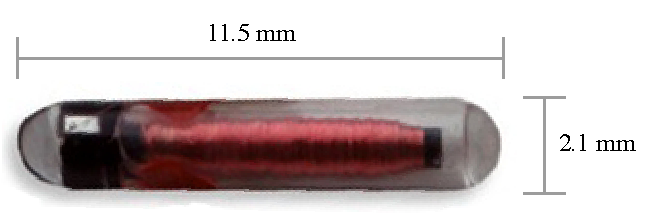
\includegraphics[width=0.5\textwidth]{assets/pdf/transponder.pdf}
  \caption[Trovan ID-100A Microtransponder]{A Trovan ID-100A Microtransponder. The transponder weighs 0.1 g and is coated with biocompatible glass. \footnotesize Picture courtesy of Trovan.}
  \label{fig:transponder}
\end{center}
\end{figure}
\begin{figure}[htpb]
\begin{center}
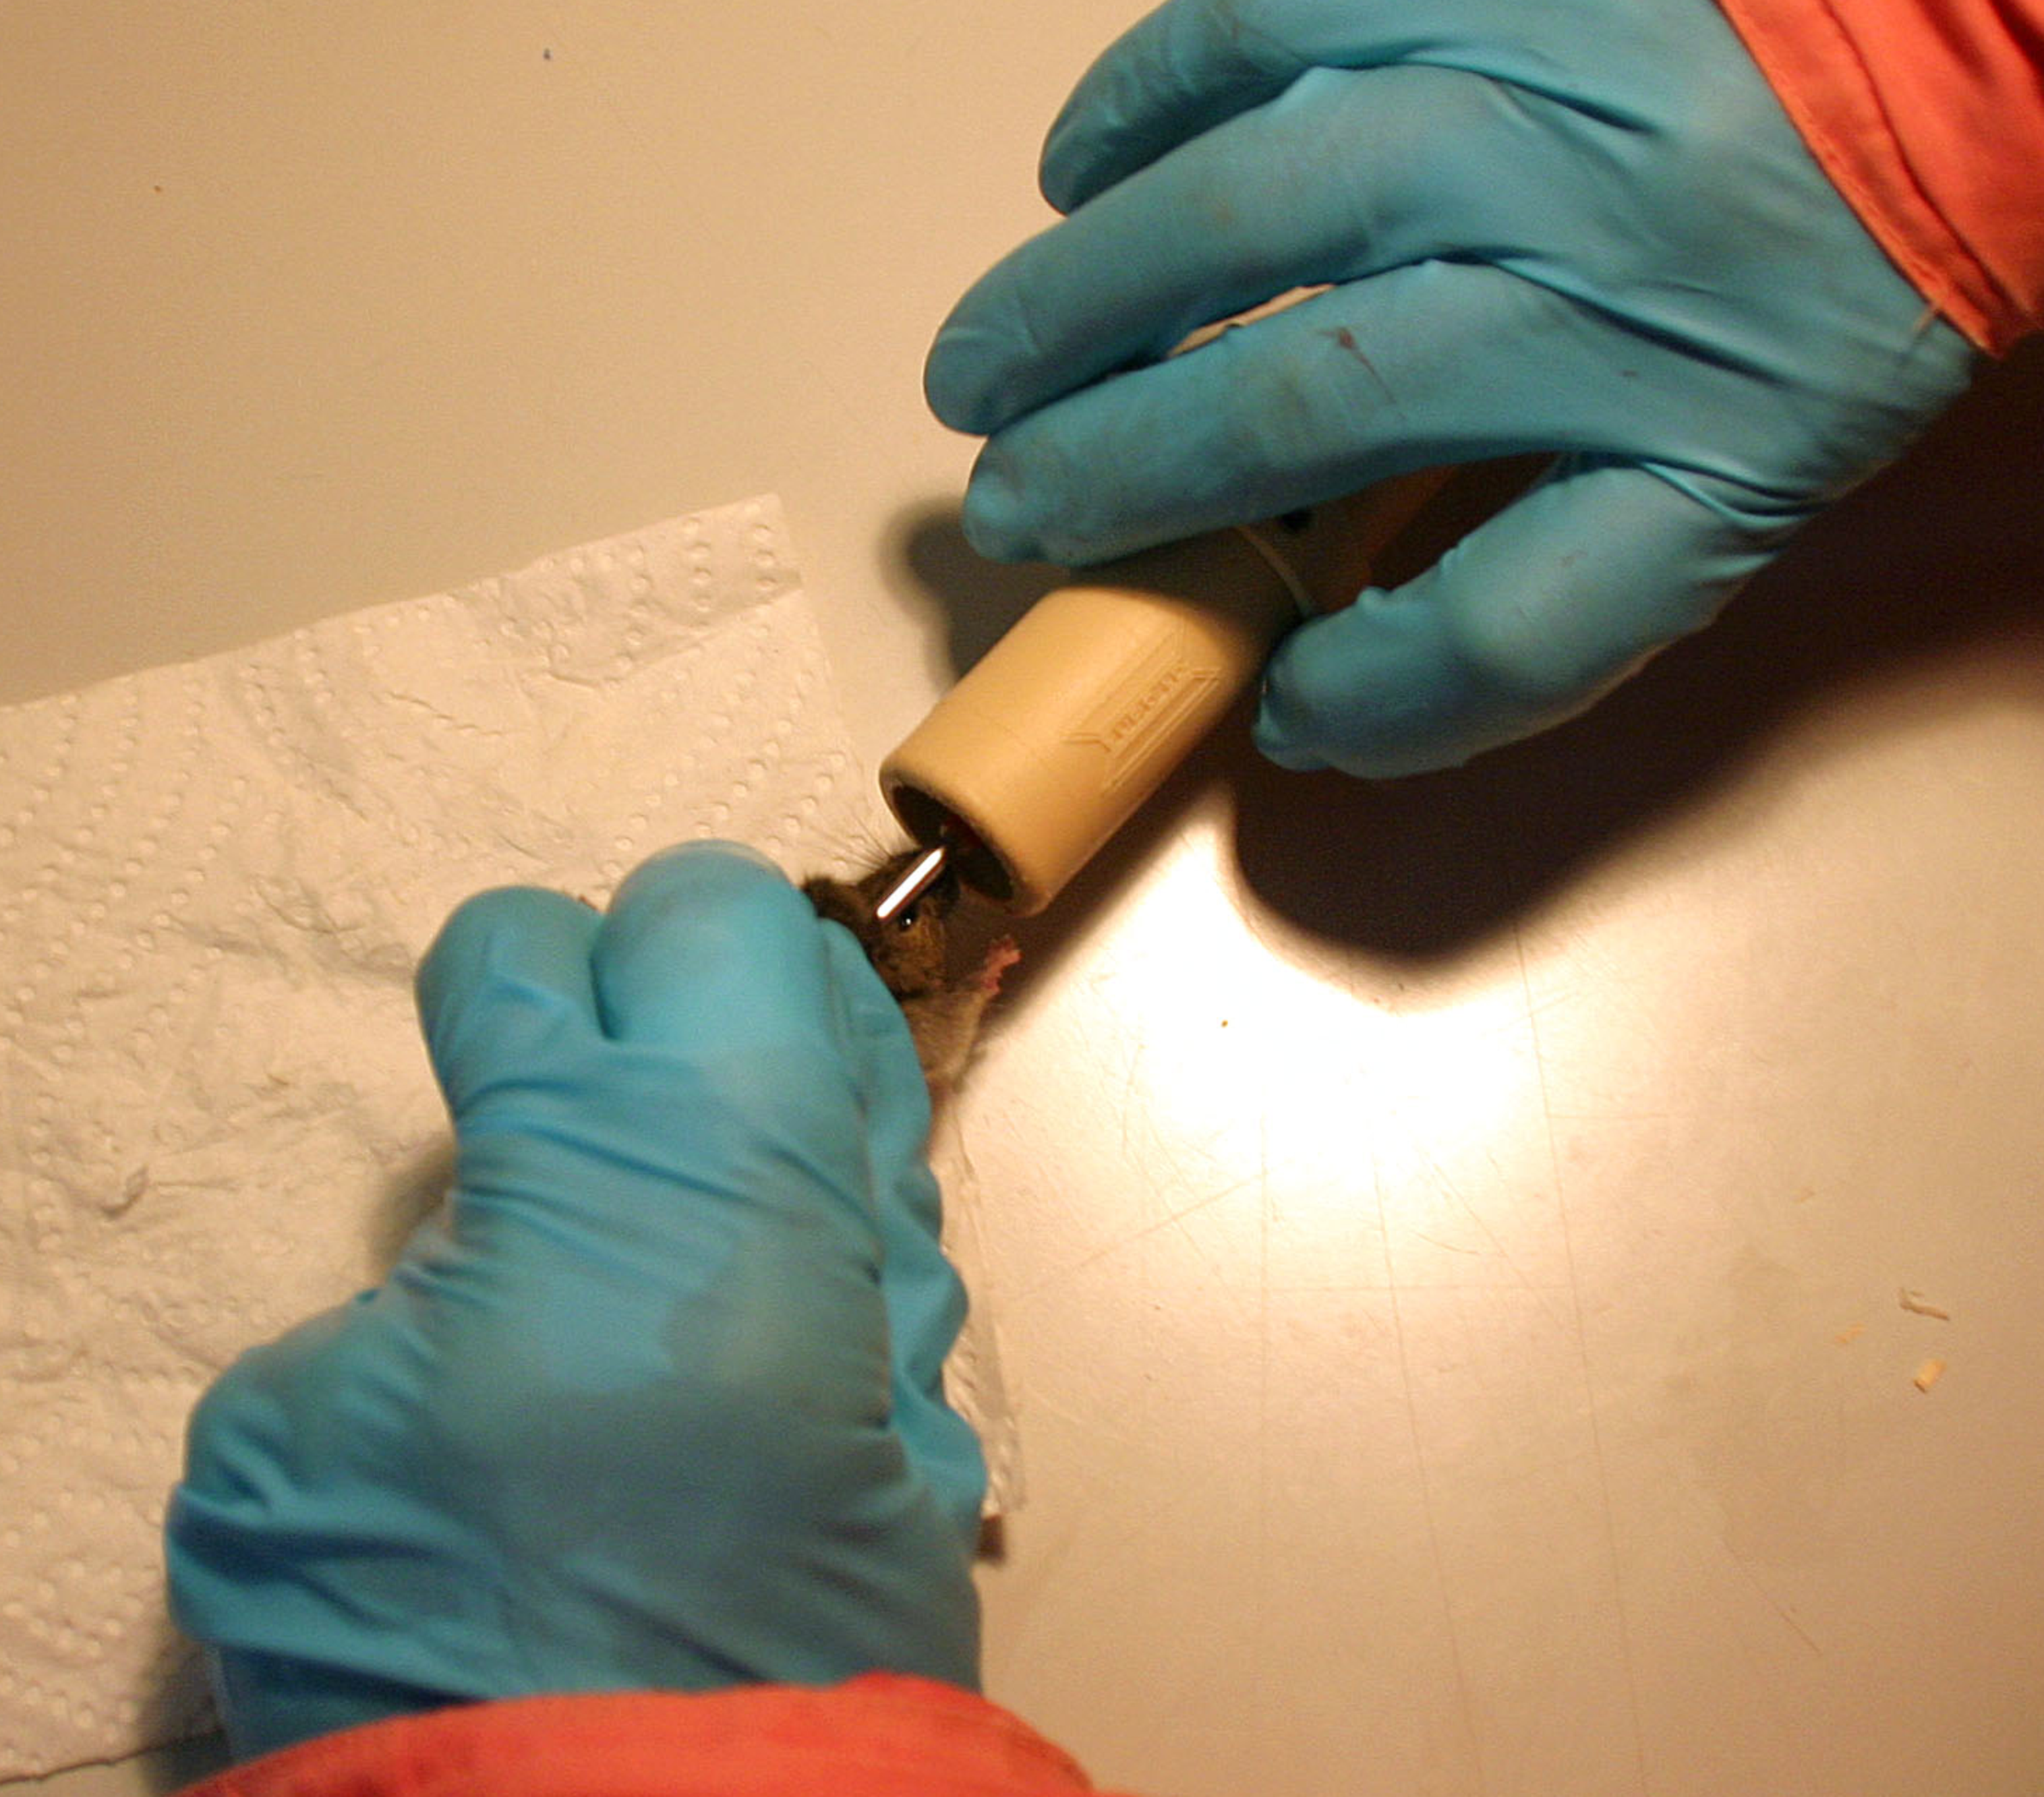
\includegraphics[width=0.5\textwidth]{assets/pdf/transponder_inject.pdf}
  \caption[Injecting an RFID transponder]{Subcutaneous injection of an RFID transponder.}
  \label{fig:inject_rfid}
\end{center}
\end{figure}

Furthermore, tissue samples are taken from the ear of each individual for genetic analysis. The genetic information provides an insight into the relatednesses within the mice population and allows to compare specific genetic markers. Genotype information is not included in the data used for this thesis.

%----------------------------------------------
%Position / Time data
% ----------------------------------------------
\subsection{Collecting spatial position data}
\label{subsec:collectspatialpos}

To collect the spatial position data, a project-specific system has been by built by \textit{New Behaviour}, a company specialized in developing technical systems to study animal behavior. 

The basic idea is to identify mice carrying an RFID transponder at specific locations. The locations where the identification occurs are the 40 artifical nestboxes distributed in the barn. 

An artificial nestbox consists of a cylinder, made of \ac{PVC}, with diameter and height of 15 cm and an entry tube made of \textit{Plexiglas}, which is about 20 to 25 cm long. Wrapped around the tube are two antennas with a coverage radius of 10 to 12 cm, capable of reading out the RFID transponders. Each antenna can be identified by an address which is set manually. To improve the antenna accuracy, the entry tube is bent 45 degrees to slow down the mice passing through. Figure \ref{fig:artNestbox} depicts a model of such an artificial nestbox.

\begin{figure}[htbp]	
\centering	
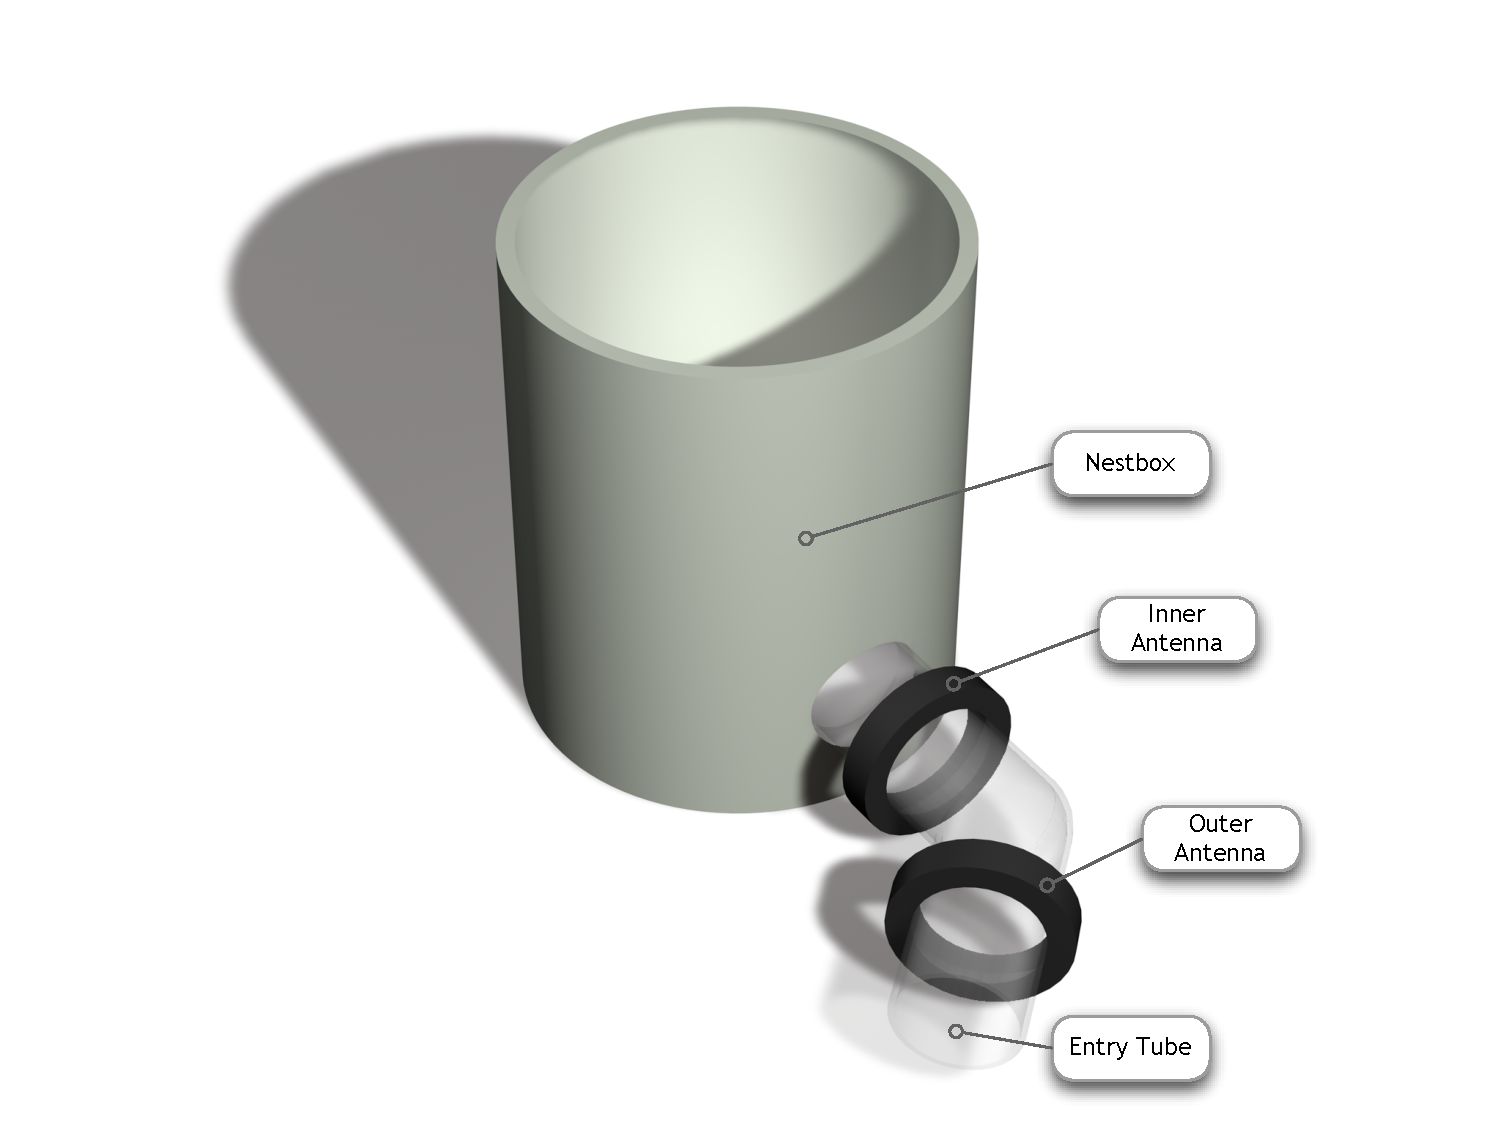
\includegraphics[width=0.75\textwidth]{assets/pdf/box_schema.pdf}	
\caption[Model of an artificial nestbox]{3D-Model of an artificial nestbox with the two antennas wrapped around the entry tube.}
\label{fig:artNestbox}
\end{figure}

The RFID transponders used are passive, meaning that they do not include a battery. The antenna acts as a scanner, presenting an inductive field that excites the transponder within antenna range. This energy is used by the transponder to send its identification to the antenna. 

Therefore, whenever a mouse carrying a transponder passes by an antenna, its identification is recorded and sent to a central computer along with the antenna address. The computer then adds a time value to the received data before writing it to a text file. The structure of these text files containing the data is detailed in the next section.

\subsubsection{Data file format}
\label{subsubsec:datafileformat}
The data files are simple text files, where each line denotes an event registered by an antenna in the system. Every day the data file is saved, closed, and a new one is created automatically by the system.

There are to types of events: %Bullets! -tnetter 09/09/2009 15:35 % rico - how do put that in a list without a point at the end? 
\begin{mylist}
 \item The first type occurs if the antenna could identify a transponder. In such a case a line as shown in figure \ref{fig:dataset} is written to the data file. The id of the transponder is a unique, ten character wide, alphanumeric value
 \item The second type of event, for which the resulting data line looks as shown in Fig. \ref{fig:dataset_no_data}, occurs when a transponder enters or leaves the coverage area of an antenna
 \item 
\end{mylist}

\begin{figure}[!htbp]	
\centering	
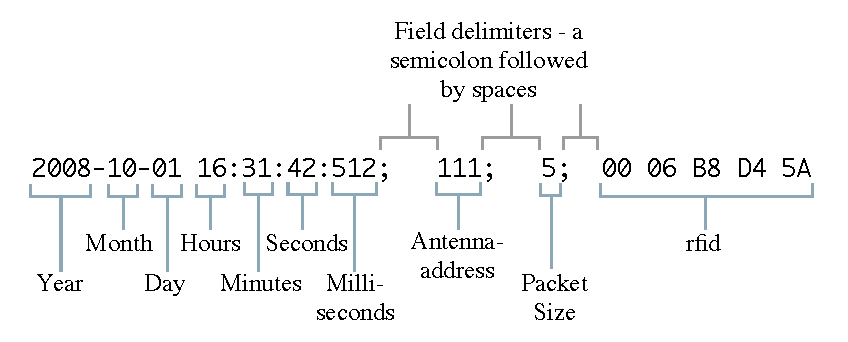
\includegraphics[width=0.6\textwidth]{assets/pdf/dataset.pdf}	
\caption[Dataset including an RFID transponder identification]{Typical dataset in a data file including an RFID transponder identification.}
\label{fig:dataset}
\end{figure}

\begin{figure}[!htbp]	
\centering	
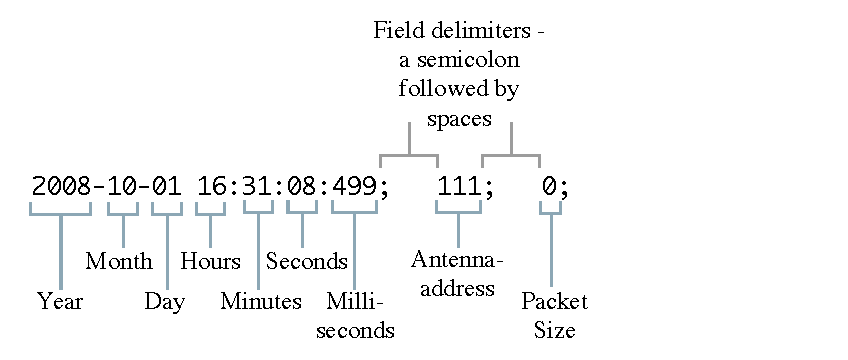
\includegraphics[width=0.6\textwidth]{assets/pdf/dataset_no_data.pdf}	
\caption[Dataset without RFID transponder identification]{Typical dataset in a data file without an RFID transponder identification.}
\label{fig:dataset_no_data}
\end{figure}

\needspace{9\baselineskip}
The following clipping and corresponding list show the data generated when a transponder passes by a nestbox. The events are explained in the subsequent list.  

\numcodestyle
\begin{lstlisting}[frame=none]
2008-10-01 16:31:08:499;   111;   0; 
2008-10-01 16:31:09:095;   113;   0; 
2008-10-01 16:31:42:512;   111;   5;  00 06 B8 D4 5A
2008-10-01 16:31:42:807;   113;   5;  00 06 B8 D4 5A
2008-10-01 16:31:43:619;   111;   0; 
2008-10-01 16:31:44:014;   113;   0;
\end{lstlisting}

The list numbering matches the line numbering of the clipping.  

\begin{condensed_enum}
  \item Transponder \textbf{enters coverage area} of the antenna with address \lstinline|111|.
  \item Transponder \textbf{enters coverage area} of the antenna with address \lstinline|113|.
  \item Transponder is \textbf{identified} as \lstinline|00 06 B8 D4 5A| at antenna with address \lstinline|111|.
  \item Transponder is \textbf{identified} as \lstinline|00 06 B8 D4 5A| at antenna with address \lstinline|113|.
  \item Transponder \textbf{leaves coverage area} of the antenna with address \lstinline|111|.
  \item Transponder \textbf{leaves coverage area} of the antenna with address \lstinline|113|. 
\end{condensed_enum}

Depending on the event type, the value of the packet size is either a \lstinline|0|, for events without a transponder identification value, or a \lstinline|5| if the transponder has been identified. For the data processing (see section \ref{sec:dataproc} on page \pageref{sec:dataproc}) only the datasets with a transponder identification are taken into account.

\subsubsection{Antenna addressing}
\label{subsubsec:addressing}

The antenna address is three digits long, composed of the box number it is attached to (first two digits) and the position at the entry tube of the box. Outer antennas have a \lstinline|1| as the last digit of the address, inner antennas a \lstinline|3| (e.g the antennas attached to box 11 are addressed 111 for the outer, 113 for the inner antenna, respectively). Needless to say, box numbers must be unique.

Unfortunately there are a few exceptions to that schema, as for a few antennas the correct addressing failed due to technical problems (see section \ref{subsec:problems}).

% \subsubsection{General system design and functionality}
% \label{subsubsec:generalsystem}
% 
% \begin{itemize}
%   \item Can-Bus
%   \item cable loop
%   \item rfid identification how
%   \item What happens in the boxes (boards) next to the antennas
%   \item How is can bus working/implemented
%   \item Where are the different cable loops (which antennas connected to a loop)
%   \item General system layout (cabling, protocols)
%   \item Programmed software
%   \item etc. 
% \end{itemize}

% ----------------------------------------------
%Data attributes
% ----------------------------------------------
\subsection{Collecting Data Attributes}
\label{subsec:dataattr}

During the \textit{population checks}, the whole barn, including all nestboxes, plastic pipes, and other structuring elements, is checked to collect mice attribute data according to the following procedure:

\begin{enumerate} 
\item Each box is opened and the following observations made:
\begin{mylist}
      \item \textbf{Mice in the box:} If adult mice are in the box, they get identified by their transponder, measured, and weighed. Furthermore we check whether the sex of the mouse has already been determined.  
      \item \textbf{Bedding:} Determine if the nestbox shows marks of use, like trampled bedding.
      \item \textbf{Nest:} Determine whether the nestbox contains an open or closed nest built by the mice out of hay or straw regularly provided in the barn.  
      \item \textbf{Pups:} Does the box contain pups, and if yes how many and what is their estimated age. 
      \item \textbf{Communal nest:} Check if two or more litters are reared in the box. 
    \end{mylist}
\item All the possible shelters, like planks and pipes, are checked for mice presence as well.
\end{enumerate}

% ----------------------------------------------
%storing Data
% ----------------------------------------------
\subsection{Data storage}
\label{subsec:datastorage}

This section details the design of the database. Data is stored in a \textit{MySQL}\footnote{\href{http://www.mysql.com/}{MySQL database}} database, which is  a \acf{RDBMS} (RDBMS). Figure \ref{fig:database_schema} on page \pageref{fig:database_schema} in the appendix shows an overview of all tables, including the data types\footnote{An overview of the MySQL data types can be found at: \url{http://dev.mysql.com/doc/refman/5.0/en/data-types.html}} of the columns and their relationship to columns in other tables.

Upon completion of a cascade of \ac{perl} scripts that process and extract information from the spatial position data in the data files, the resulting data is merged with the collected attribute data and is written to the tables as outlined in here. For details about the cascade refer to section \ref{sec:dataproc}. 

The tables can be split up in three different groups, depending of the sort of data they contain. 

\subsubsection{Processed data}

This group covers tables exclusively written to by the scripts in the import cascade. A diagram of the tables belonging to that group, as well as the relations between them, is shown in figure \ref{fig:processed_data_schema}. 

\begin{figure}[htpb]
\begin{center}
  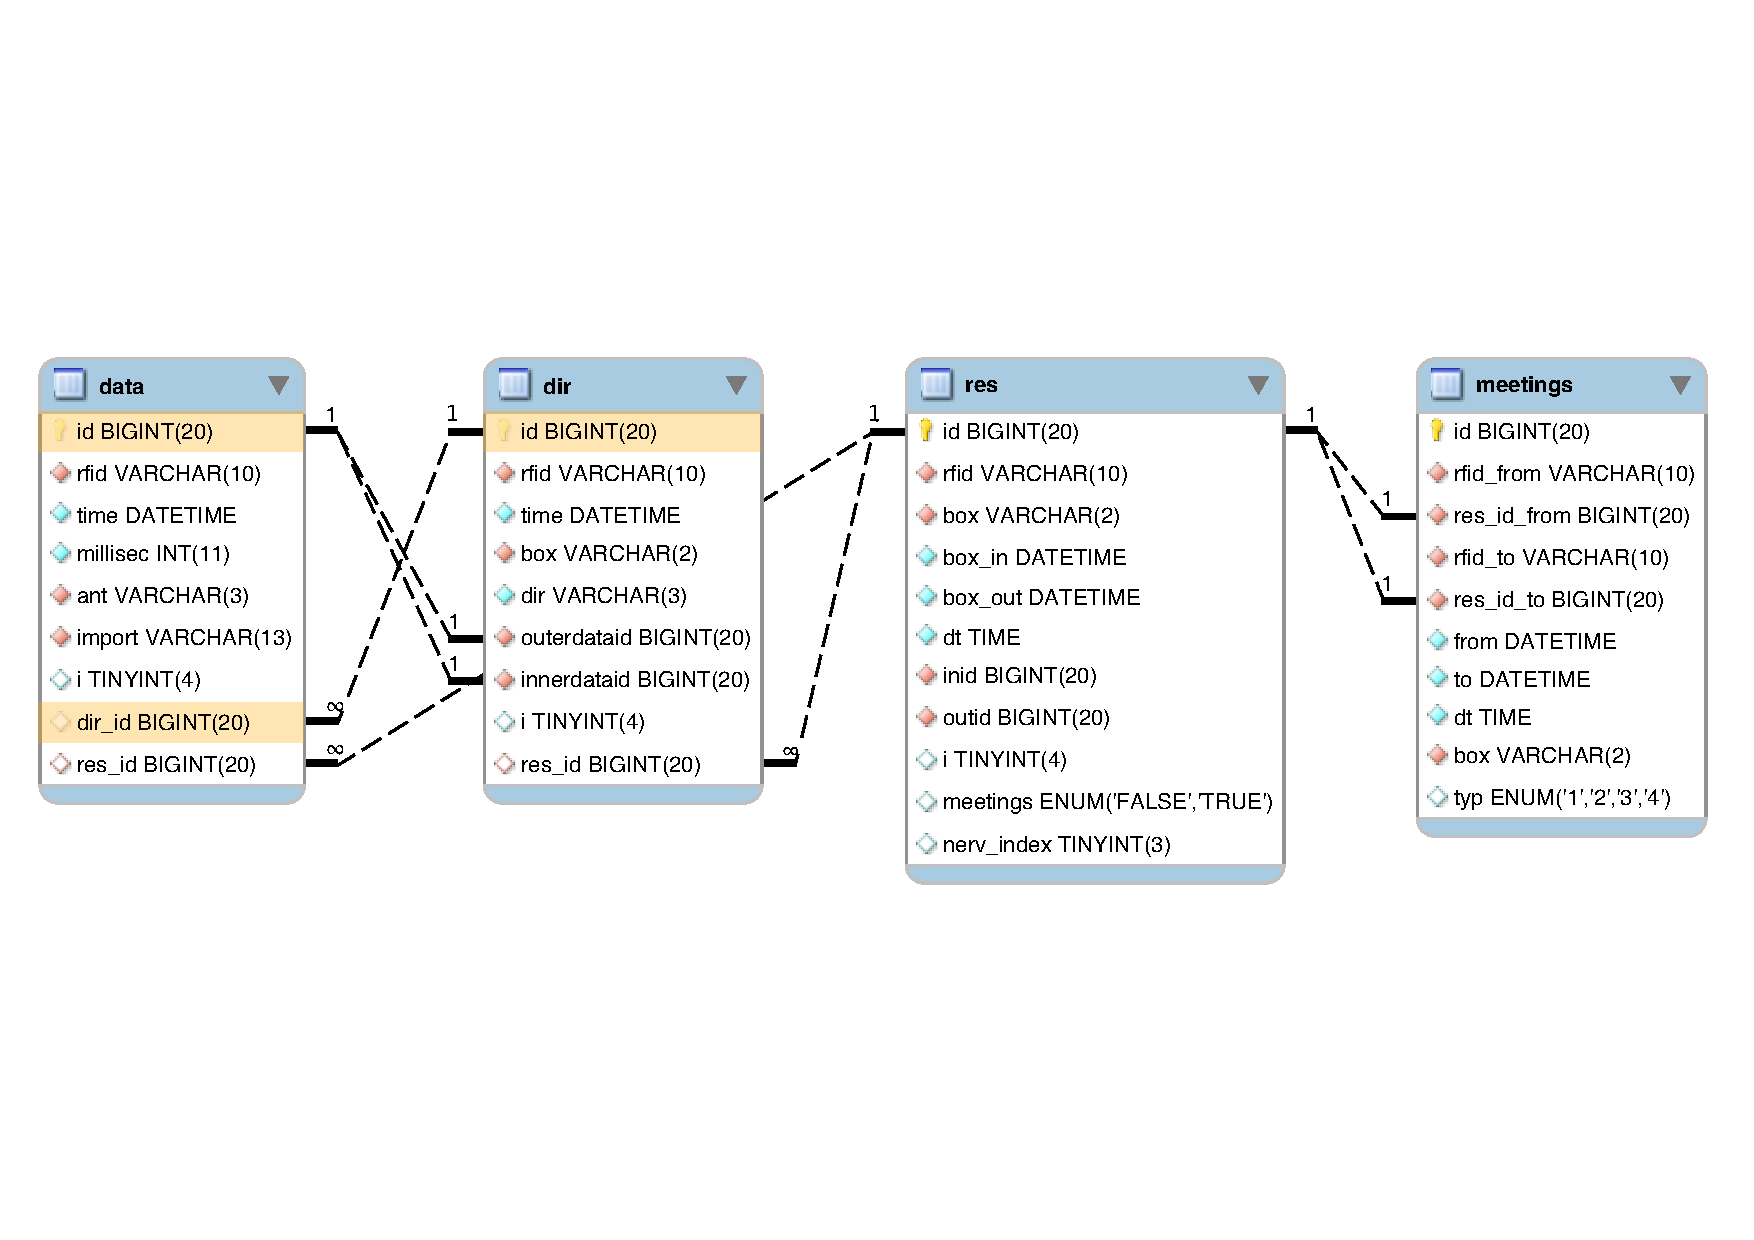
\includegraphics[width=\textwidth]{assets/pdf/processed_data_schema.pdf}
  \caption[Diagram of database tables with processed data]{Diagram of the database tables with the processed spatial position data and the relations between them.}
  \label{fig:processed_data_schema}
\end{center}
\end{figure} 

\paragraph{data table}
\label{para:data_table}

A script (see section \ref{subsec:importing}) imports the data files written by the antenna system in the barn into the \lstinline|data| table.

Shown next is a row of the \lstinline|data| table followed by short explanation of the columns.

\codescript
\needspace{14\baselineskip}
\begin{lstlisting}[frame=none]

(first part of table row)
+---------+------------+---------------------+----------+
| id      | rfid       | time                | millisec |
+---------+------------+---------------------+----------+
| 7321019 | 00069B4D4D | 2009-02-07 00:51:56 |      173 |
+---------+------------+---------------------+----------+

(second part of table row)
+-----+---------------+------+--------+--------+
| ant | import        | i    | dir_id | res_id |
+-----+---------------+------+--------+--------+
| 121 | 09-0206155809 |    4 |  40102 |  10001 |
+-----+---------------+------+--------+--------+

\end{lstlisting}

\begin{mydesc}
  \item \lstinline|id| is a unique identifier of a dataset in this table. Such a unique identifier is normally used as target for a relation between columns of different tables and does not have any further meaning.
  \item \lstinline|rfid| is a transponder value. This value is a reference to a value in the \lstinline|id| column of the \lstinline|rfid| table (see section \ref{para:rfid_table}).
  \item \lstinline|time| and \lstinline|millsec| columns harbor the time the dataset has been recorded. Unfortunately the \textit{MySQL} \lstinline|DATETIME| data type does not include the milliseconds. Hence, these values have to be stored in a separate column.
  \item \lstinline|ant| denotes the antenna the data was recorded at. This value is a reference to a value in the \lstinline|id| column of the \lstinline|ant| table (see section \ref{para:ant_table}).
  \item \lstinline|import| is a reference to a dataset with an equivalent value of \lstinline|short| in the \lstinline|logs| table (see section \ref{para:logs_table}), simply unveils of which data file this dataset is part of.
  \item \lstinline|i| is an indicator if the dataset could be used in a \lstinline|direction result| and \lstinline|stay result| (see \ref{para:res_table}). Table \ref{tab:i_values} on page \pageref{tab:i_values} of the appendix gives an overview of the meaning of the \lstinline|i| values in the different tables.
  \item \lstinline|dir_id| is a reference to an \lstinline|id| in the \lstinline|dir| table, if that dataset could be used in a \textit{direction result}. Else, this value is \lstinline|NULL|\footnote{\textit{MySQL} sets the \lstinline|NULL| value to indicate a missing or unknown value.}.
  \item \lstinline|res_id| is a reference to an \lstinline|id| in the \lstinline|res| table, if that dataset could be used in a \textit{stay result}. Else this value is \lstinline|NULL|.
\end{mydesc}

\paragraph{dir table}
\label{para:dir_table}

Another script (see section \ref{subsec:dirres}) searches for matching pairs of datasets in the \lstinline|data| table which form a \textit{direction result}. When a mouse carrying a transponder passes the two antennas attached to the nestbox's entry tube, it is possible within a given time to determine if the mouse went in or out of that box. 

Shown next is a row of the \lstinline|dir| table followed by a short explanation of the columns.

\codescript
\needspace{14\baselineskip}
\begin{lstlisting}[frame=none]

(first part of table row)
+-------+------------+---------------------+-----+-----+
| id    | rfid       | time                | box | dir |
+-------+------------+---------------------+-----+-----+
| 40102 | 00069B4D4D | 2009-02-07 00:51:56 | 12  | in  |
+-------+------------+---------------------+-----+-----+

(second part of table row)
+-------------+-------------+------+--------+
| outerdataid | innerdataid | i    | res_id |
+-------------+-------------+------+--------+
|     7321019 |     7321020 |    4 |  10001 | 
+-------------+-------------+------+--------+
\end{lstlisting}

\begin{mydesc}
  \item \lstinline|id| and \lstinline|rfid| have the identical function as in the \lstinline|data| table.
  \item \lstinline|time| denotes the moment the the \lstinline|rfid| entered or left the \lstinline|box|.
  \item \lstinline|box| is a reference to a value in the \lstinline|id| column of the \lstinline|box| table (see section \ref{para:box_table}).
  \item \lstinline|dir| is either set to \lstinline|in| or \lstinline|out| and depicts the direction.
  \item \lstinline|outerdataid| and \lstinline|innerdataid| values can be used to backtrack the datasets in the \lstinline|data| table making up the \textit{direction result}. This is explained in detail in section \ref{subsec:dirres} on page \pageref{subsec:dirres}.
  \item \lstinline|i| is an indicator if the direction result could be used in a \textit{stay result} (see \ref{para:res_table}). Table \ref{tab:i_values} on page \pageref{tab:i_values} of the appendix gives an overview of the meaning of the \lstinline|i| values in the different tables.
  \item \lstinline|res_id| is a reference to an \lstinline|id| in the \lstinline|res| table, if that dataset could be used in a \textit{stay result}. Else this value is \lstinline|NULL|.
\end{mydesc}

\paragraph{res table}
\label{para:res_table}

When two \textit{direction results} are found (one with a \lstinline|dir| value of \lstinline|in| and the other with a \lstinline|dir| value of \lstinline|out|, as well as matching \lstinline|rfid| and \lstinline|box| values), they form a so called \textit{stay result}.

Shown next is a row of the \lstinline|res| table followed by a short explanation of the columns.

\codescript
\needspace{14\baselineskip}
\begin{lstlisting}[frame=none]

(first part of table row)
+-------+------------+-----+---------------------+---------------------+
| id    | rfid       | box | box_in              | box_out             |
+-------+------------+-----+---------------------+---------------------+
| 10001 | 00069B4D4D | 12  | 2009-02-07 00:51:56 | 2009-02-07 00:52:01 |
+-------+------------+-----+---------------------+---------------------+

(second part of table row)
+----------+-------+---------+------+----------+------------+
| dt       | inid  | outid   | i    | meetings | nerv_index |
+----------+-------+---------+------+----------+------------+
| 00:00:05 | 40102 | 7321021 |    4 | TRUE     |          1 | 
+----------+-------+---------+------+----------+------------+

\end{lstlisting}

\begin{mydesc}
\item \lstinline|id|, \lstinline|rfid| and \lstinline|box| were already explained for the previous tables, and have the same function in this table.
\item \lstinline|box_in| and \lstinline|box_out| denote the arrival and departure times of an \lstinline|rfid| in a \lstinline|box|.
\item \lstinline|dt| denotes the duration of the result, equal to the time elapsed between \lstinline|box_in| and \lstinline|box_out|.
\item \lstinline|inid| and \lstinline|outid| can be used to backtrace the datasets in the \lstinline|dir| or \lstinline|data| table making up the \textit{stay result}.
\item \lstinline|i| is either \lstinline|3| or \lstinline|4| and indicates the type of result. This distinction is explained in section \ref{subsec:stayres}.
\item \lstinline|meetings| is set to \lstinline|true| when the result set has been analyzed for meetings (see next paragraph and section \ref{subsec:meetingres} for details about the \textit{meeting results}).
\item \lstinline|nerv_index| gives an idea about how \textit{nervous} the mouse was when it stayed in the box. Details about this value can be found in section \ref{subsec:stayres} as well.
\end{mydesc}

\paragraph{Meetings table}
\label{para:meetings_table}

In this work, an event is termed a \textit{meeting}, if \textit{stay results} of different mice in the same box show a temporal overlap. The meeting data is written to the \lstinline|meetings| table.

Shown next is a row of the \lstinline|meetings| table followed by a short explanation of the columns.

\codescript
\needspace{14\baselineskip}
\begin{lstlisting}[frame=none]

(first part of table row)
+--------+------------+-------------+------------+-----------+
| id     | rfid_from  | res_id_from | rfid_to    | res_id_to |
+--------+------------+-------------+------------+-----------+
| 302635 | 0006CD478F |      596630 | 0006CC7962 |    596100 | 
+--------+------------+-------------+------------+-----------+

(second part of table row)
+---------------------+---------------------+----------+-----+------+
| from                | to                  | dt       | box | typ  |
+---------------------+---------------------+----------+-----+------+
| 2009-03-27 16:58:36 | 2009-03-27 17:01:00 | 00:02:24 | 13  | 1    |
+---------------------+---------------------+----------+-----+------+
\end{lstlisting}

\begin{mydesc}
\item \lstinline|id| is again the unique identifier.
\item \lstinline|rfid_from| and \lstinline|rfid_to| denote the two participating RFID's (mice) of the \textit{meeting result}.
\item \lstinline|res_id_from| points to the \lstinline|id| of the \textit{stay result} from the \lstinline|rfid_from|, and the \lstinline|res_id_to| to the one of the \lstinline|rfid_to|. This allows to look up the \textit{stay results} making up this \lstinline|meeting result|.
\item \lstinline|from|, \lstinline|to| and \lstinline|dt| declare the meeting's start and end times, as well as duration.
\item \lstinline|box| contains the reference to an \lstinline|id| in the \lstinline|box| table (see section \ref{para:box_table}).
\item The different values of the \lstinline|typ| column are detailed in section \ref{subsec:meetingres}.
\end{mydesc}

\subsubsection{System members data}
\label{subsubsec:system_members_tables}

This group encloses the tables which contain information about the RFID's (transpondered mice) as well as the antennas and boxes.

Figure \ref{fig:system_members} shows an overview of the tables within this group plus the relations between the table columns. 

\begin{figure}[htpb]
\begin{center}
  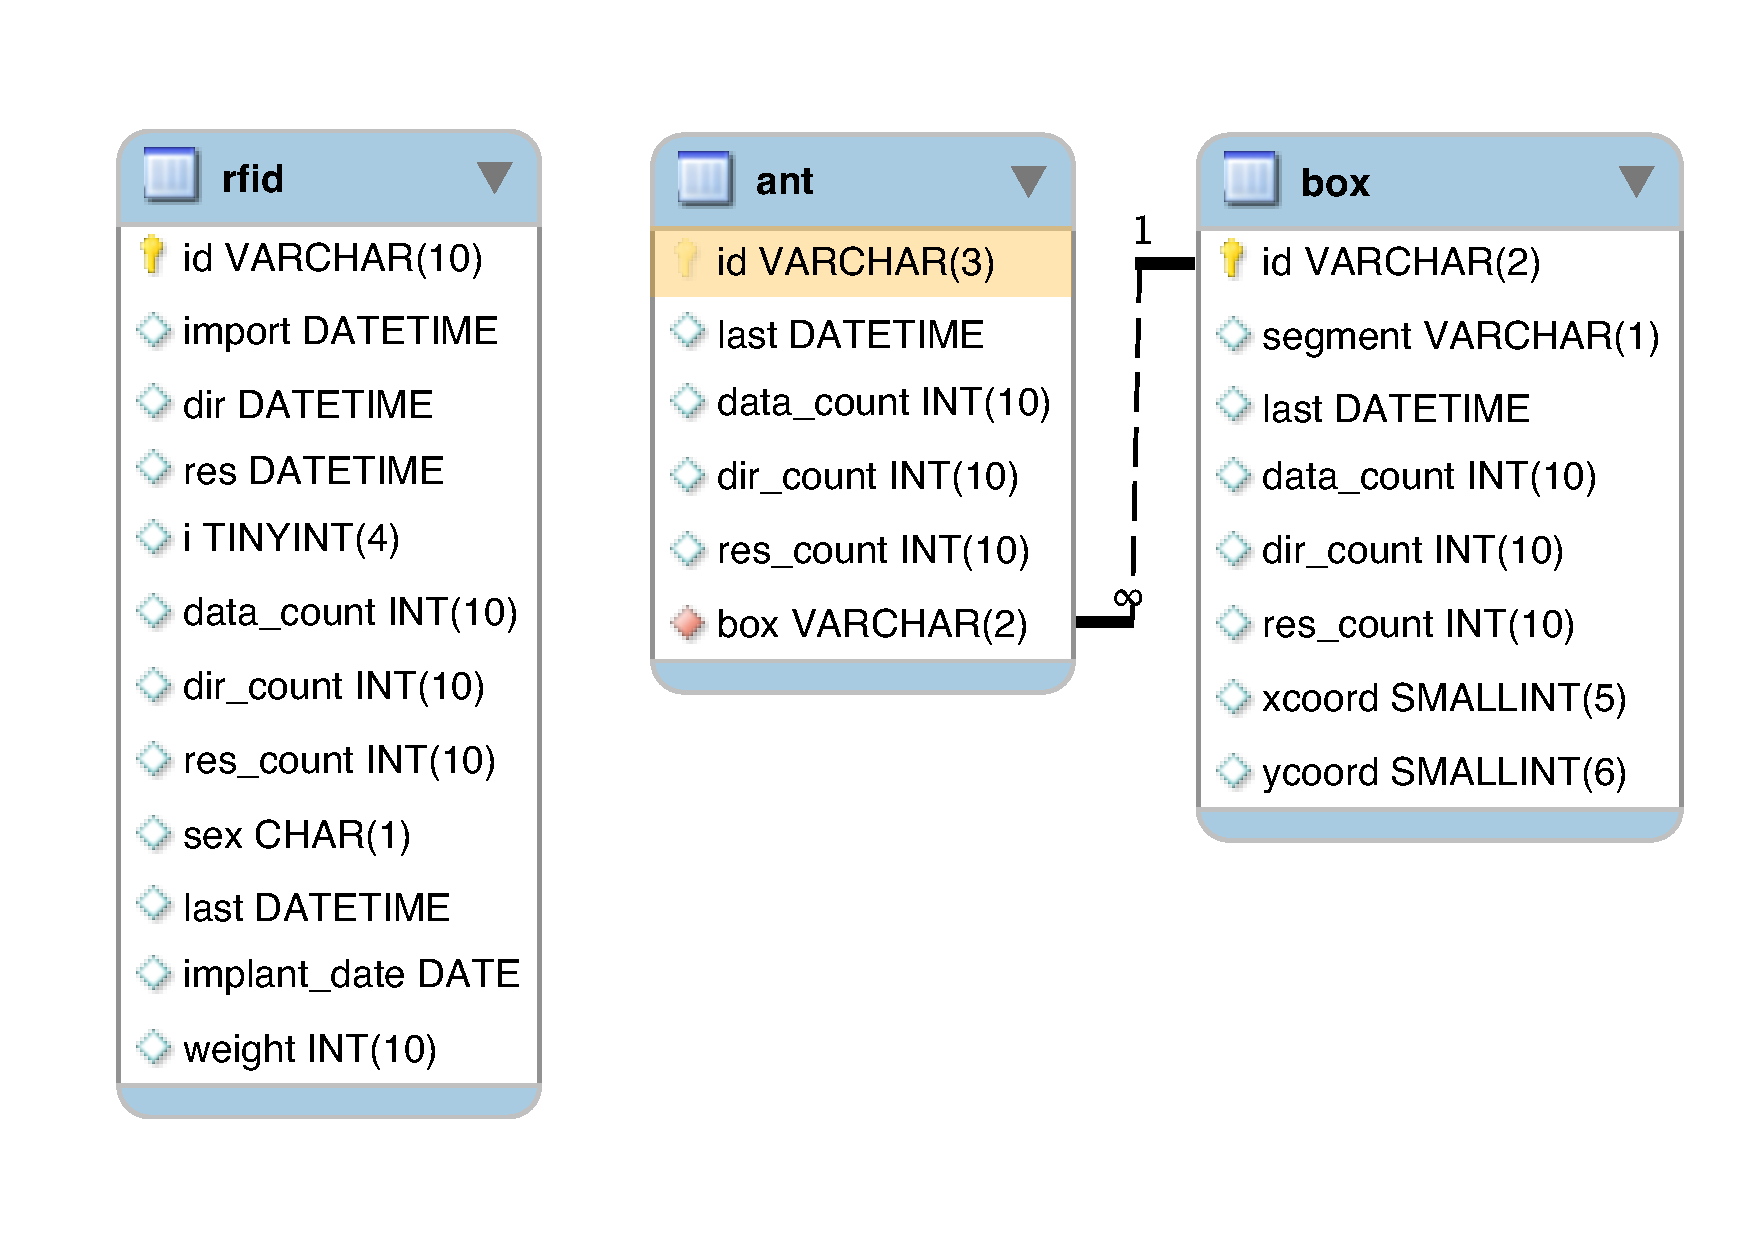
\includegraphics[width=0.75\textwidth]{assets/pdf/system_members_schema.pdf}
  \caption[Schema of database tables with system member data]{Schema of the database tables containing the \textit{system members} data.}
  \label{fig:system_members}
\end{center}
\end{figure}

\paragraph{rfid table}
\label{para:rfid_table}

All the RFID's ever recorded by the system, including their corresponding attribute data, are stored in the \lstinline|rfid| table.

Shown in the next listing is a row of the \lstinline|rfid| table followed by short a explanation of the columns.
\codescript
\needspace{14\baselineskip}
\begin{lstlisting}[frame=none]

(first part of table row)
+------------+------+------------+-----------+-----------+
| id         | i    | data_count | dir_count | res_count |
+------------+------+------------+-----------+-----------+
| 0006955EED |    3 |          1 |         0 |         0 |
+------------+------+------------+-----------+-----------+

(second part of table row)
+------+---------------------+--------------+--------+
| sex  | last                | implant_date | weight |
+------+---------------------+--------------+--------+
| m    | 2007-08-29 23:35:41 | 2007-08-28   |   18.0 |
+------+---------------------+--------------+--------+

\end{lstlisting}

\begin{mydesc}
\item \lstinline|id| is the unique, 10 character wide, alphanumeric RFID transponder identification.
\item \lstinline|i| is is a helper value used in the data import procedure. It is \lstinline|0| if new data for the transponder has been imported, \lstinline|2| if the data is searched for \textit{direction results} and \lstinline|3| if the data has been searched for \textit{stay results}.
\item \lstinline|data_count| contains the sum of datasets in the \lstinline|data| table.
\item \lstinline|dir_count| contains the sum of datasets in the \lstinline|direction| table.
\item \lstinline|res_count| contains the sum of datasets in the \lstinline|results| table.
\item \lstinline|sex| denotes the gender of the mouse, when known.
\item \lstinline|last| points to the maximum value in the \lstinline|time| column of the \lstinline|data| table for this mouse, which is just the last time the transponder has been recorded by the antenna system.
\item \lstinline|implant_date| holds the date of the RFID tag's hypodermic injection.
\item \lstinline|weight| contains a decimal number with the weight of the mouse in grams.
\end{mydesc}

\paragraph{box table}
\label{para:box_table}

The box table contains all the information about the 40 nestboxes. 

Shown next is a row of the \lstinline|box| table followed by a short explanation of the columns.
\codescript
\needspace{14\baselineskip}
\begin{lstlisting}[frame=none]

(first part of table row)
+----+---------+---------------------+------------+
| id | segment | last                | data_count |
+----+---------+---------------------+------------+
| 01 | A       | 2009-03-27 16:38:59 |     122439 | 
+----+---------+---------------------+------------+

(second part of table row)
+-----------+-----------+--------+--------+
| dir_count | res_count | xcoord | ycoord |
+-----------+-----------+--------+--------+
|     44389 |      9824 |    246 |    708 | 
+-----------+-----------+--------+--------+

\end{lstlisting}

\begin{mydesc}
\item \lstinline|id| is the unique 2 character wide box identification.
\item \lstinline|segment| points to the segment (A, B, C or D) the box is located in.
\item The meaning of the \lstinline|last|, \lstinline|data_count|, \lstinline|dir_count| and \lstinline|res_count| columns was already explained in the \lstinline|rfid| table.
\item \lstinline|xcoord| and \lstinline|ycoord| denote the position of the nestbox in the barn. The x-axis stands for the entrance wall and the y-axis for  the side wall to the left of the entrance. The coordinate values are stored in centimeters. 
\end{mydesc}

\paragraph{ant table} 
\label{para:ant_table}

The ant table contains all the information about the 80 antennas. 

Shown next is a row of the \lstinline|ant| table followed by a short explanation of the columns.
\codescript
\needspace{14\baselineskip}
\begin{lstlisting}[frame=none]
+-----+---------------------+------------+-----------+-----------+-----+
| id  | last                | data_count | dir_count | res_count | box |
+-----+---------------------+------------+-----------+-----------+-----+
| 011 | 2009-03-27 16:38:59 |      54220 |     46099 |     19648 | 01  | 
+-----+---------------------+------------+-----------+-----------+-----+

\end{lstlisting}

\begin{mydesc}
\item \lstinline|id| is the unique 3 character wide antenna address.
\item The meaning of the \lstinline|last| \lstinline|data_count|, \lstinline|dir_count| and \lstinline|res_count| columns was already explained in the \lstinline|rfid| table.
\item \lstinline|box| points to the \lstinline|id| value in the \lstinline|box| table, the antenna is attached to.
\end{mydesc}

\subsubsection{Auxiliary tables}
\label{subsubsec:auxiliary_tables}

Tables in this group contain data about the imported data files, and precalculated values to improve the performance when browsing the data using the graphical user interface (which is introduced in section \ref{subsec:dataexp}).

Figure \ref{fig:auxiliary_tables} shows an overview of the tables within this group. 


\begin{figure}[htpb]
\begin{center}
  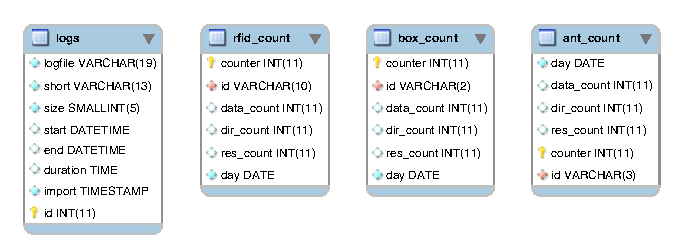
\includegraphics[width=0.75\textwidth]{assets/pdf/auxiliary_tables_schema.pdf}
  \caption[Schema of database tables with system member data]{Schemata of the database tables with the auxiliary data.}
  \label{fig:auxiliary_tables}
\end{center}
\end{figure}

\paragraph{logs table}
\label{para:logs_table} 

The \lstinline|logs| table contains information about the imported data files.

Shown next is a row of the \lstinline|logs| table followed by a short explanation of the columns.

\codescript
\needspace{14\baselineskip}
\begin{lstlisting}[frame=none]
(first part of table row)
+-----+---------------------+---------------+------+---------------------+
| id  | logfile             | short         | size | start               |
+-----+---------------------+---------------+------+---------------------+
| 608 | 20090326_170750.txt | 09-0326170750 | 1660 | 2009-03-26 17:07:51 |
+-----+---------------------+---------------+------+---------------------+

(second part of table row)
+---------------------+----------+---------------------+
| end                 | duration | import              |
+---------------------+----------+---------------------+
| 2009-03-27 17:07:40 | 23:59:49 | 2009-04-12 01:03:01 | 
+---------------------+----------+---------------------+

\end{lstlisting}

\begin{mydesc}
\item \lstinline|id| is the unique identifier of dataset.
\item The original filename of the data file is stored in the \lstinline|logfile| column.
\item \lstinline|short| values are a kind of code made up from parts of the data filename. This column was important at the beginning of the project, when we had to import data files with another file format.
\item \lstinline|size| contains the filesize, in bytes, of the data file.
\item \lstinline|start| and \lstinline|end| indicate the file's first and last record timestamps.
\item \lstinline|duration| is simply the period between the \lstinline|start| and \lstinline|end| values.
\item \lstinline|import| is the data import into \lstinline|data| completion timestamp
\end{mydesc}

\paragraph{RFID\_count, box\_count, ant\_count}
\label{para:counts}

These three tables contain the per day data counts for transponders (\lstinline|rfid_count|), boxes (\lstinline|box_count|), and antennas (\lstinline|ant_count|). They are only needed by the user interface to speed up data browsing.

Shown next is a row of the \lstinline|rfid_count|, \lstinline|box_count|, \lstinline|ant_count| tables followed by a short explanation of the columns.

\codescript
\needspace{14\baselineskip}
\begin{lstlisting}[frame=none]
(row of table rfid_count)
+---------+------------+------------+------------+-----------+-----------+
| counter | id         | day        | data_count | dir_count | res_count |
+---------+------------+------------+------------+-----------+-----------+
|     999 | 0006B9C5E8 | 2008-07-14 |         10 |         4 |         2 | 
+---------+------------+------------+------------+-----------+-----------+


(row of table box_count)
+---------+----+------------+------------+-----------+-----------+
| counter | id | day        | data_count | dir_count | res_count |
+---------+----+------------+------------+-----------+-----------+
|     999 | 10 | 2008-07-31 |        259 |       114 |        39 | 
+---------+----+------------+------------+-----------+-----------+


(row of table ant_count)
+---------+-----+------------+------------+-----------+-----------+
| counter | id  | day        | data_count | dir_count | res_count |
+---------+-----+------------+------------+-----------+-----------+
|     999 | 121 | 2008-07-19 |        196 |       174 |        47 | 
+---------+-----+------------+------------+-----------+-----------+


\end{lstlisting}

\begin{mydesc}
\item \lstinline|counter| is the unique dataset identifier.
\item \lstinline|id| contains the \lstinline|id| value of the transponder, the box or the antenna.
\item \lstinline|day| points to the day the table row holds the data counts for.
\item \lstinline|data_count|, \lstinline|dir_count| and \lstinline|res_count| contain the per day counts for the datasets, the \textit{direction results} and the \textit{stay results}.
\end{mydesc}

\subsection{Efficiency and problems of the antenna system}
\label{subsec:problems}

Unfortunately the problems with the antenna system are diverse such as antenna drop outs, broken laptop or cable connections chewed by mice, to name just a few. Some of these problems could be solved.

However, one of the biggest problem is that the readings at the antennas are not as reliable as expected. This is clearly visible by looking at the efficiency of the system , measured by comparison of theoretical and actual number of \textit{direction} and \textit{say results}. 

From the 5th of April 2007 to the 27th of March 2009, approximately 8 million datasets (table \lstinline|data|)  
have been collected. Theoretically we would get around 4 million \textit{direction results}. The actual number of \textit{directio  results} is 2.9 million. The exact percentage is 71.16\%.

In the next step, two \textit{direction results} should create a \textit{stay result}. The script which searches for the \textit{stay results} could find 1.5  results in the 3 million \textit{direction results}, but finds around one million. More exactely  68.25\%. Most likely these low numbers are an effect of missed antenna readings.
 
Normally, an antenna reads the RFID tag 10 times to increase a reading's reliability. The antenna system in the barn, however, reads the RFID only 3 times, as the time that a tagged mouse spends within antenna range is usually short. We can partly understand the impact of shortened sampling duration by looking at the \lstinline|rfid| table. The table contains 4605 different transponder id's, whereby only 1014 have been sampled over 10 times. The other 3546 rfids are most probably a result of a phenomenon called \textit{bit flipping}.

The following listing shows an excerpt of a data file, where a RFID tag is identified as \lstinline|00 05 B8 D2 70| on line two, but as \lstinline|00 06 B8 E2 70| on the other lines. 

\numcodestyle
\needspace{5\baselineskip}
\begin{lstlisting}[frame=none]
2007-11-25 10:09:12:906;   381;   5;  00 06 B8 E2 70
2007-11-25 10:09:16:529;   381;   5;  00 05 B8 D2 70
2007-11-25 10:09:16:932;   381;   5;  00 06 B8 E2 70
2007-11-25 10:09:19:950;   381;   0; 
2007-11-25 10:09:20:253;   381;   5;  00 06 B8 E2 70
\end{lstlisting}

The first four digits of the transponder identification represent the manufacturer's serial number. The manufacturer sold us only RFID's from the \lstinline|00 06| series. Because of this we can conclude that line two is a read error. Still, this transponder has been read 53 times between November 2007 and May 2008, but none of the readings could be used to form a \textit{direction result}. Assuming that this is not a singular case, we get many of these false readings which lead to a low subsequent data processing yield. 

Furthermore, for some antennas the address could not be set properly. In one case two antennas even sent the same address, so that distinction of the data is impossible. The workaround for this problem is to find an unused address which we are able to set, and map it to the desired address during data import (see section \ref{subsec:importing}).   

\subsection{Data access}
\label{subsec:dataccess}

Most of the mainly used relational databases offer \ac{SQL} (SQL) to manage and retrieve data. However, SQL is not easy to learn and use, lacks built-in export functionality to file formats such as \textit{Microsoft Excel}, and does not offer the possibility to visualize data. We therefore provide a feature-rich and intuitive \acf{GUI} (GUI) to facilitate exploration, visualization, and data export. A presentation of the GUI can be found in section \ref{sec:dataaccessandexp}.